\documentclass[11pt,a4paper]{article}
% \usepackage[brazil]{babel} % carrega portugues brasileiro
\usepackage[utf8]{inputenc}
\usepackage[T1]{fontenc}
\usepackage[top=2cm, bottom=2cm, left=2cm, right=2cm]{geometry} %margens menores!
\usepackage{graphicx} % incluir figuras .eps
\usepackage{tabularx}
\usepackage{color} % colorir texto
\usepackage{indentfirst}
\usepackage{textcomp}
\usepackage[colorlinks=true]{hyperref}
\usepackage{amssymb,amsmath}
\usepackage{float}
% \usepackage{siunitx}
% \usepackage[ampersand]{easylist}

\title{HERMES - High-frequency Emergency and Rural Multimedia Exchange
  System Software Description}

\author{
       \large
        \textsc{Rafael Diniz}
        \mbox{}\\ %
        rafael@rhizomatica.org\\
        \mbox{Rhizomatica} \\ %
%        \normalsize
%        \texttt{Brasília - Brasil}\\
}
\date{\today}


\begin{document}

\maketitle

\begin{abstract}

This document describes the software stack of the HERMES (High-frequency Emergency and Rural Multimedia Exchange System)
- a digital communication system for the HF band which uses a
high-performance HF modem and UUCP networking (Unix to Unix
Communication Protocol), for email transport and other ad-hoc
services. HERMES is also composed of email software infrastructure and
Web Interface for access to the services, which run on a computer.

\end{abstract}

\newpage

\tableofcontents

\section{Introduction}

  Telecommunication in the HF Band using skywave propagation offers hundreds to thousands
  of kilometers coverage with relative low power and simple antennas, but it is also challenging,
  given the extreme limitation on throughtput  and very long transceiver turn-around times between tx and rx.

  HERMES is a digital telecommunication system for the HF band, which uses a high-performance HF modem and UUCP
  (Unix-to-Unix Communication Protocol), for email transport and other ad-hoc services.
  UUCP is arguably the most relevant store-and-forward system to date, in use since the late 70's
  for software exchange, email, bulletin board systems  news and even military communication. First released
  in Bell Labs' Unix Version 7, it is still present in all major Unixes (including Linux) and integrate seamless
  with email software like Postfix.

  Upper network layers are composed by email software infrastructure and Web Interface for management and access to the services.
  HERMES network topology is flexible, but tipically configured as star, with a ``gateway'' station located where Internet is available
  (in order to route data from stations located in isolated areas) and ``remote'' stations located at communities without access to
  other telecommunication systems.

%  While not a requirement at the time of development, UUCP lacks basic security and supports no encryption. HERMES,
%  on the other hand, is being used by indigenous communities in vulnerable contexts, in which encryption is a must-have.
%  While HERMES already provide some level of security, as individual messages can be encrypted, through the use of e-mail encryption,
%  all metadata is transported in clear, including the UUCP connection establishment and authentication procedures. This revised proposal
%  to NLNet involves adding security and encryption to UUCP, without the need for extra layers and extensive overhead (like using UUCP
%  over ssh over IP, which is not feasible in HF given the amount of tx/rx switches and huge overhead).

\section{HERMES Description}

This section briefly introduces what HERMES system can do today. HERMES is basically composed of:

\begin{itemize}
\item HF transceiver and associated antenna, connected to a computer;
\item Computer running the HERMES free software stack;
\item The computer provides local connectivity through WiFi (or other local-area network
  technology)
\end{itemize}

Rhizomatica developed the HERMES hardware which embedds all the needed parts for a simple to use
HF telecomunication equipment. Figure~\ref{fig1} and ~\ref{fig2} contains a picture of the HERMES box. The HERMES box contains
everything needed for joining a HERMES network, while users have access to the HERMES services over WiFi or ethernet.


\begin{figure}[h!]
  \centering
  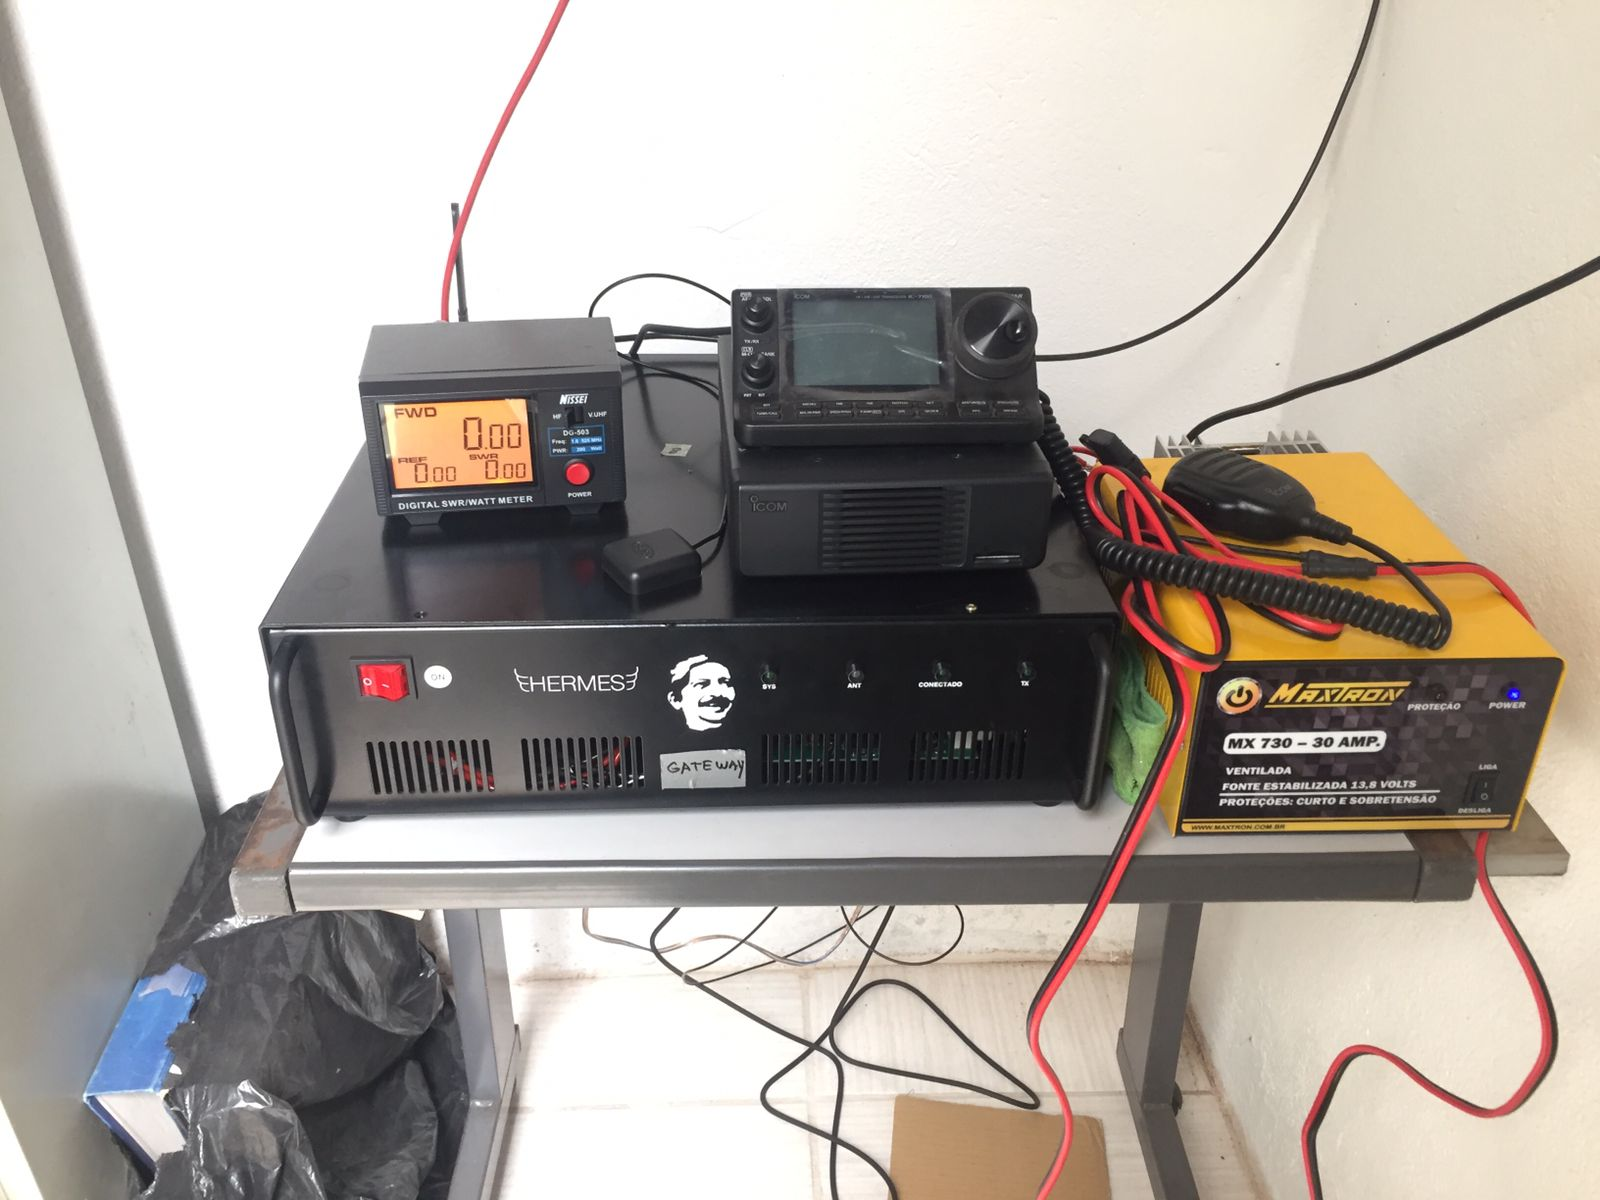
\includegraphics[scale=0.15]{hermes-pic1.jpeg}
  \caption{The HERMES hardware at a ``gateway'' location, a power supply (yellow), a standard HF voice radio (top right) and a wattmeter (top left).}
  \label{fig1}
\end{figure}

\begin{figure}[h!]
  \centering
  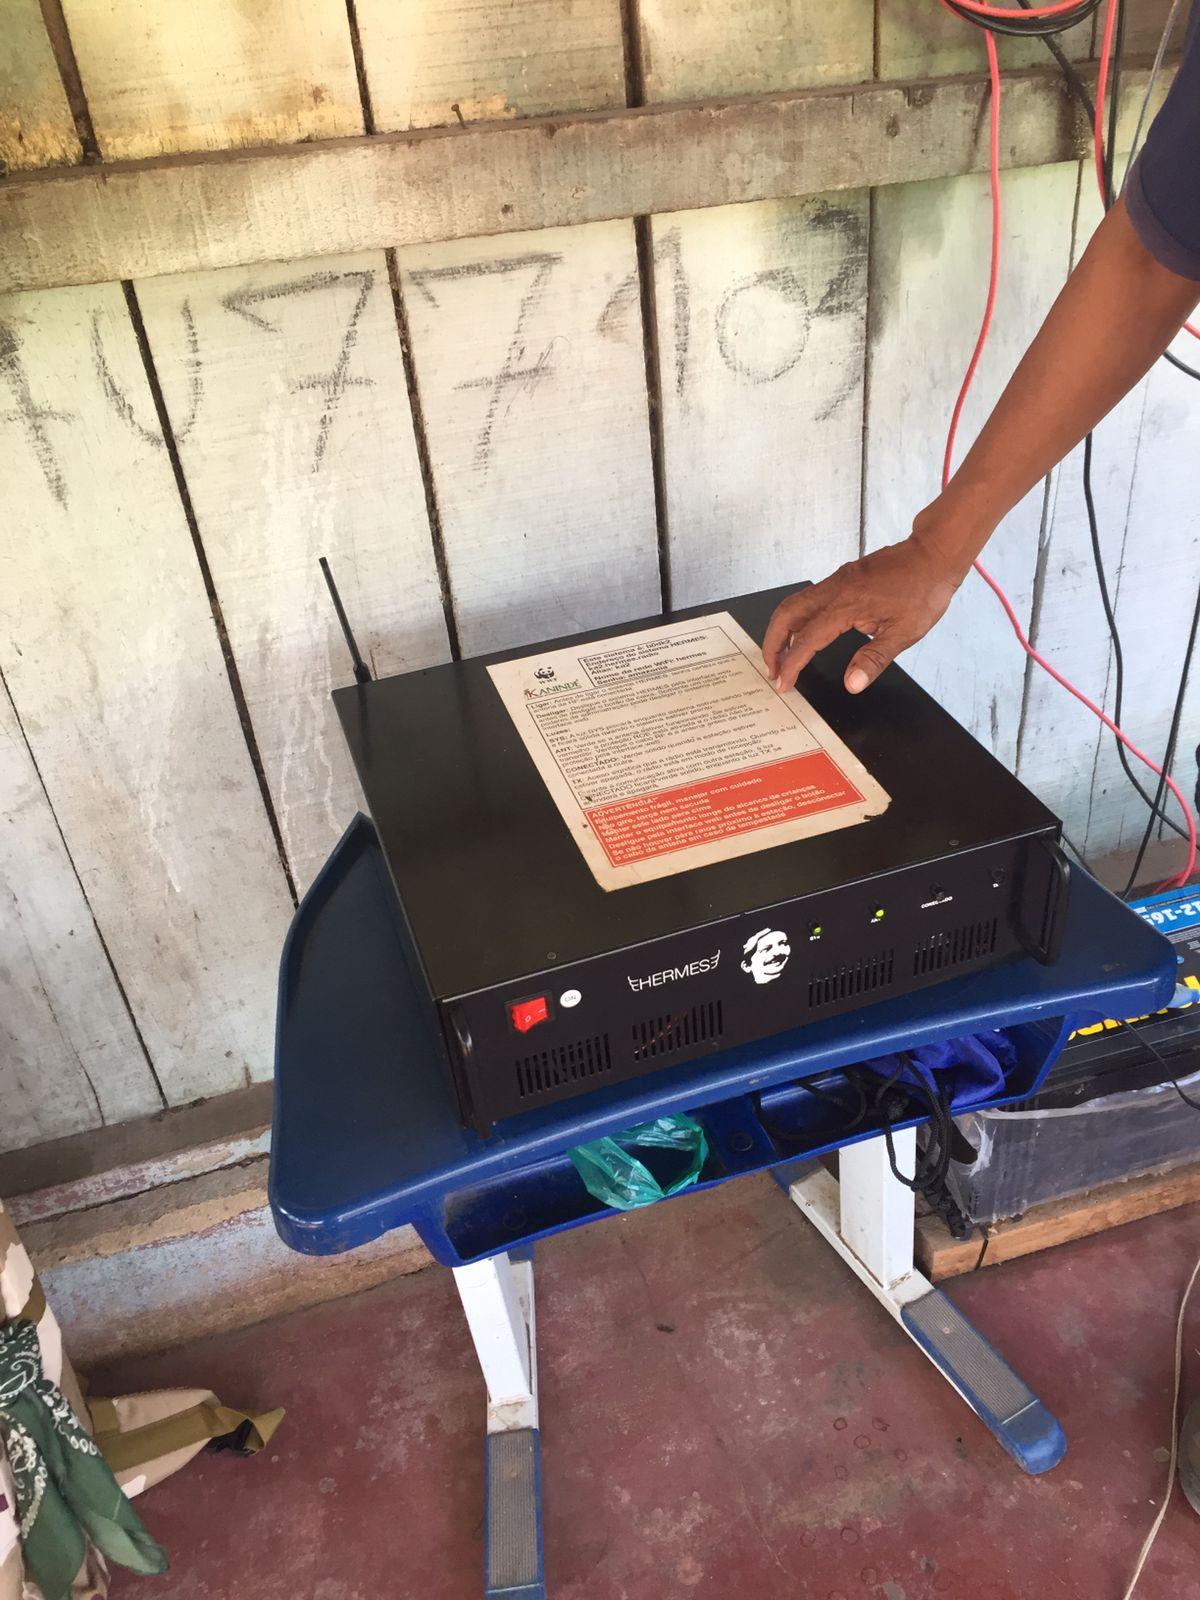
\includegraphics[scale=0.15]{hermes-pic2.jpeg}
  \caption{The HERMES hardware at a ``remote'' location, with a battery appearing the bottom left.}
  \label{fig2}
\end{figure}


HERMES uses GNU UUCP with Debian downstream patches (version 1.07-27 or greater, available at: \url{https://packages.debian.org/bullseye/uucp}).

Specific HERMES network stack source code, radio firmware and other system components are available at:

\begin{itemize}
\item Main network components and firmware: https://github.com/Rhizomatica/hermes-net
\item REST API: https://github.com/Rhizomatica/hermes-api
\item Web GUI: https://github.com/Rhizomatica/hermes-gui
\item Documentation: https://github.com/Rhizomatica/hermes-documentation
\end{itemize}


\section{HERMES Software Stack}

HERMES uses ARDOP (Amateur Radio Digital Open Protocol) or VARA for modem. ARDOP and VARA are
SDR (software defined radio) modems which use modern modulation techniques (OFDM) and support
standard HF transceiver specification (up to 3 kHz bandwidth).

For the network layer, UUCP is used. UUCP is a system for asynchronous
store-and-forward communication first released in Bell Labs Unix V7 in
the late 1970s, and still used today in niches, like communication over HF.

The uucpd (previously called rhizo-uuardop) project was developed to provide
integration between UUCP and the HF modem.

The HERMES network stack is made of:
\begin{itemize}
\item HF Radio Transceiver
\item ALSA (Audio/Signal configuration)
\item HF Modem (Modem configuration)
\item UUCP (Network configuration)
\item UUCPD (UUCP / HF Modem connection tools)
\item Email (Email stack configuration)
\item Graphical Web-based User Interface
\end{itemize}

\subsection{HF Radio Transceiver}

TODO (what follows is old text... prior to HERMES hardware development)

Different setups require different configuration. In the case of using a USB
(Universal Serial Bus) interface (e.g. Signalink), the delay must be set to
0. In the case of radios with USB connection exposed an embedded sound
card and transmit/receive control (eg. ICOM IC-7100) set the bandpass
filter to at least 2.8kHz (or wider) for digital operation (SSB/Data).

\subsection{ALSA (Audio configuration)}

Add to ``/etc/asound.conf'':
\begin{verbatim}
pcm.ARDOP {type rate slave {pcm "hw:1,0" rate 48000}}
\end{verbatim}

Where ``hw:1,0'' is the HF transceiver's audio device.

\subsection{ARDOP (Modem configuration)}

Download link: \url{https://github.com/DigitalHERMES/ardopc}

The ardop binary should be in /usr/bin/ardop, which can be a
symbolic link to /usr/bin/{ardop1ofdm, ardop2, ardopofdm}.

ARDOP service file for the ICOM IC-7100 (USB connection, PTT done over serial):
\begin{verbatim}
[Unit]
Description=ARDOP daemon

[Service]
Type=simple
ExecStart=/usr/bin/ardop 8515 -c /dev/ttyUSB0 ARDOP ARDOP -k FEFE88E01C0001FD -u FEFE88E01C0000FD
ExecStop=/usr/bin/killall -s QUIT ardop
IgnoreSIGPIPE=no
#StandardOutput=null
#StandardError=null
StandardOutput=syslog
StandardError=syslog

[Install]
WantedBy=multi-user.target
\end{verbatim}

Service file when using a VOX based setup (eg. when using an interface like
the Signalink):
\begin{verbatim}
[Unit]
Description=ARDOP daemon

[Service]
Type=simple
ExecStart=/usr/bin/ardop 8515 ARDOP ARDOP
ExecStop=/usr/bin/killall -s QUIT ardop
IgnoreSIGPIPE=no
#StandardOutput=null
#StandardError=null
StandardOutput=syslog
StandardError=syslog

[Install]
WantedBy=multi-user.target
\end{verbatim}


Start/stop ARDOP service:
\begin{verbatim}
systemctl start ardop.service
systemctl stop ardop.service
\end{verbatim}


See the log:
\begin{verbatim}
journalctl -f -u ardop
\end{verbatim}

\subsection{UUCP (Network configuration)}

UUCP Debian package version 1.07-27 or higher should be used, for example,
the version from Debian Bullseye (11):
\url{https://packages.debian.org/bullseye/uucp}. Packages for Raspberry OS
Buster can be installed using our repository. Example for installation in a
Raspberry Zero or 1 (32bit armv6l Raspberry devices) root terminal:

\begin{verbatim}
echo deb http://www.telemidia.puc-rio.br/~rafaeldiniz/public_files/hermes-repo/ buster main \
     >> /etc/apt/sources.list
wget http://www.telemidia.puc-rio.br/~rafaeldiniz/public_files/hermes-repo/rafaeldiniz.gpg.key
apt-key add rafaeldiniz.gpg.key
apt-get update
apt-get install uucp
\end{verbatim}


UUCP command line examples follow. To copy a file to a remote host,
the following command adds a copy job to the uucp queue (``-r'' is used to
not start transmission after queuing):
\begin{verbatim}
uucp -C -r -d source.xxx AM4AAB\!/var/www/html/arquivos/${nodename}/
\end{verbatim}

Trigger the transmission of all queued jobs for host
AM4AAA:
\begin{verbatim}
uucico -S AM4AAA
\end{verbatim}

List the jobs:
\begin{verbatim}
uustat -a
\end{verbatim}

Kill a job:
\begin{verbatim}
uustat -k job
uustat -K
\end{verbatim}

See the log:
\begin{verbatim}
uulog
\end{verbatim}


\subsection{Rhizo-uuardopd (UUCP / ARDOP connection tools)}

%TODO: It seems everything uucico wrote in the end of a reception, don't get
%to the other side - connection closes and buffer get clean fast!

Two binaries should be installed: uuport (to be called by uucp) and uuardopd
which is the daemon software that connects to the ARDOP modem to start
or stop a connection. Rhizo-uuardopd manages the connection with UUCP
through uucico or uuport.

Download link: \url{http://github.com/DigitalHERMES/rhizo-uuardop}

Start/stop UUARDOPD service:
\begin{verbatim}
systemctl start uuardopd.service
systemctl stop uuardopd.service
\end{verbatim}


See the log:
\begin{verbatim}
journalctl -f -u uuardopd
\end{verbatim}

%\subsection{DHCP}

%\subsection{DNS}

%\subsection{Apache + PHP}


\subsection{User Web Interface}

HERMES provides a web-based interface which uses Angular. Source
code is located at:
(\url{https://github.com/Rhizomatica/hermes-gui/}). Current
implementation supports symmetric cryptography and audio/image compression.

% We use ``/var/www/html/arquivos'' as the default UUCP path to send
% files through the web interface.

Requirements of the user interface:

\begin{itemize}
\item ImageMagic: for image manipulation
\item VVC: Best free software low bitrate visual content compression codec: \url{https://github.com/fraunhoferhhi/}
% \item opusenc: para comprimir áudio
\item LPCNet: Best free software audio compression codec: \url{https://github.com/xiph/LPCNet}
\item GnuPG: For cryptography
\item hostapd: WiFi AP mode software
\end{itemize}

The Web interface can be accessed by typing any address in a browser
connected to the WiFi (set the DNS accordingly) or simply 10.0.0.1.

\subsection{Email}

Please refer to:
\url{https://www.linuxbabe.com/mail-server/setup-basic-postfix-mail-sever-ubuntu}

And (for DeltaChat connection):
\url{https://www.linuxbabe.com/mail-server/enable-smtps-port-465-postfix}

%ps: WORK IN PROGRESS

%Email server (MTA) can either run locally or only in a central host with
%Internet. Stations can either opt to connect to a central station on demand,
%have some pre-defined schedule, or the central station connects to the
%community stations doing a pooling, delivering and downloading emails and
%files.

%\subsection{WebPhone}

%WORK IN PROGRESS

%\url{https://gitlab.tic-ac.org/keith/webphone/wikis/hermes}

\end{document}
